\section{Introduction}
\begin{frame}
\frametitle{Introduction}
Transformers have become the predominant architecture
in foundation models due to their excellent performance
across various domains. However,
\begin{itemize}
    \item scaling these models requires substantial costs;
    \item architectural modifications typically require the entire
    model to be retrained from scratch.
\end{itemize}
% However, the substantial cost of scaling these models
% remains a significant concern.\\
% When scaling the model, its architectural modifications are introduced
% and the entire model typically requires retraining from scratch.\\
The \textbf{Tokenformer}, a natively scalable architecture that totally
leverages the attention mechanism, was proposed.
\begin{itemize}
    \item Treat model parameters as tokens and replace all linear
    projections in Transformers with token-parameter attention layers;
    \item Input tokens act as queries and model parameters as keys
    and values;
    \item Allow for progressive and efficient scaling without retraining
    from scratch;
    \item Achieve performance comparable to Transformers while
    greatly reducing the training costs.
\end{itemize}
\end{frame}

\begin{frame}
\frametitle{Transformer vs Tokenformer}
\begin{figure}[h]
    \centering
    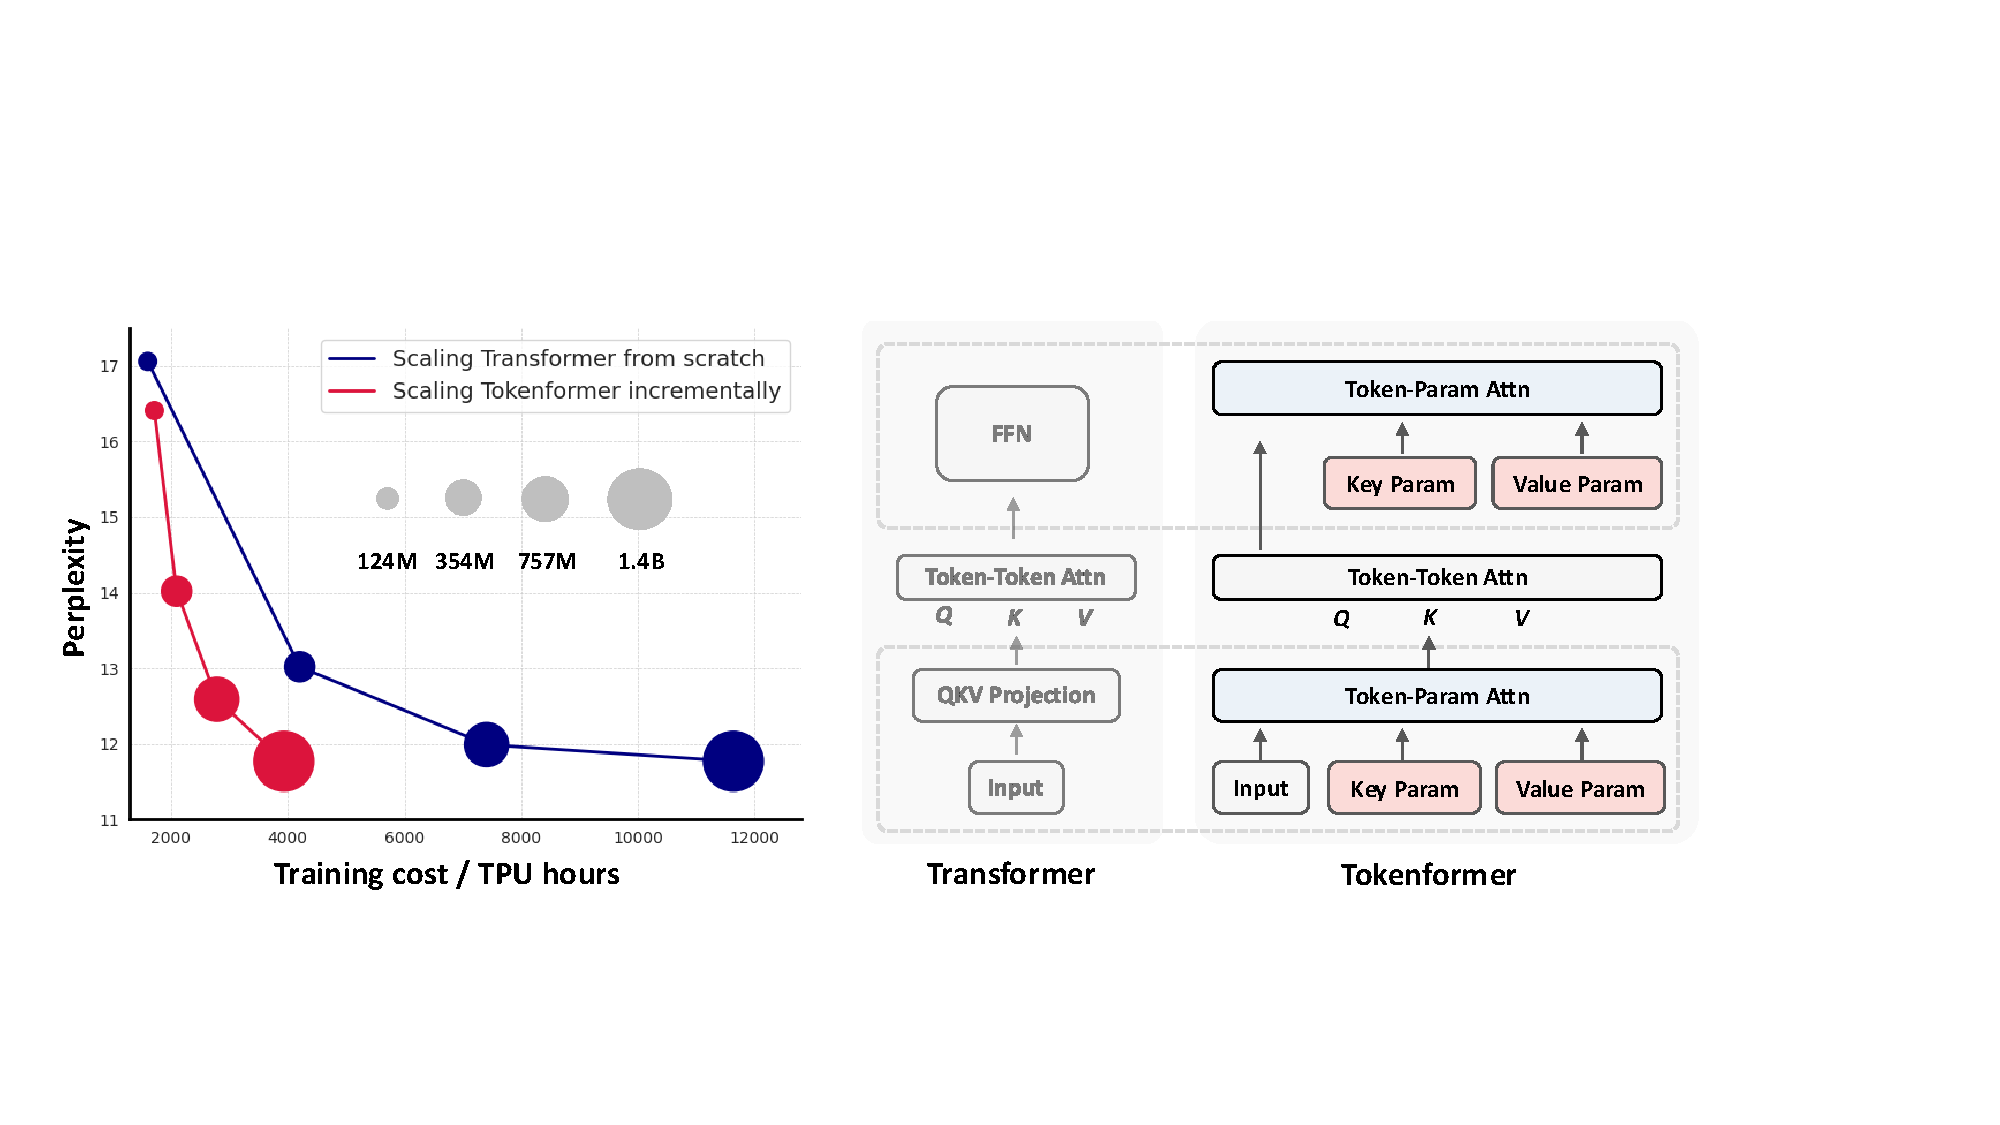
\includegraphics[width=0.99\linewidth]{./transformer-paper/intro_v4.pdf}
    \vspace{-0.1cm}
    \caption{A simple comparasion between Transformers and Tokenformers.}
    \label{fig:intro_figure}
    \vspace{-6pt}
\end{figure}
\end{frame}